\chapter{Estado del Arte}
\label{cap:estadodelarte}

El análisis del estado del arte realizado en esta tesis se agrupa en tres tipos: el primero corresponde a proyectos relacionados sobre la gestión de la producción con fabricación aditiva, el segundo sobre proyectos vinculados a la gestión del mantenimiento de equipos basados en la teoría de la confiabilidad, y el tercero en proyectos con tecnologías innovadoras que utilicen CMMS para la gestión del mantenimiento. Las palabras clave para el presente análisis son: \textit{Impresión 3D}, \textit{Fabricación aditiva}, \textit{Gestión de la producción}, \textit{gestión del mantenimiento}, \textit{CMMS}, \textit{Innovación} y \textit{Confiabilidad (RCM)}.

\section{Gestión de la producción en la fabricación aditiva}

Fera, M., Macchiaroli, R., Fruggiero, F., and Lambiase, A. (2018). Production managment fundamentals for additive manufacturing. IntechOpen

\begin{description}
\item \textbf{Objetivos:}
\begin{itemize}
\item Presentar revisión de la literatura de las principales facetas de la fabricación aditiva relacionada con el campo de la gestión de operaciones.
\item Intentar definir un modelo que de cuenta de los costos de producción y la programación de la actividad de una máquina.  
\end{itemize}
\end{description}

\begin{description}
\item \textbf{Resumen:} La manufactura aditiva es una nueva forma de producir piezas, que en los últimos años ha tenido una significativa aplicación en los ambientes tradicionales de producción, desde que ha demostrado su capacidad para producir piezas sin defectos particulares y con buenas propiedades mecánicas. Durante las dos últimas décadas, la fabricación aditiva fue primeramente usada para producir polímeros, y luego aplicada a metales; esta evolución hizo posible su entrada en los sectores industriales tradicionales, como la industria aeroespacial, mecánica y otros sectores relacionados. No obstante, la introducción de esta tecnología en el contexto mencionado anteriormente, pone en la mesa de los investigadores algunos cuestionamientos acerca de la gestión de esta tecnología en contextos más complejos, caracterizados por la integración con otras máquinas.  
\end{description}

\begin{description}
\item \textbf{Resultados:} Las palabras clave investigadas en relación a la gestión de las operaciones son \citep{fera2018}: (i) organización de la producción; (ii) equilibrio de la producción; (iii) calidad de la producción; (iv) ciclo de vida de la producción y; (v) sustentabilidad de la producción. Desde este punto de vista, la literatura analizada respecto a la gestión de operaciones utilizando manufactura aditiva no está bien cubierta aún desde el punto de vista de la investigación. Esto se puede mostrar en la siguiente figura, que muestra las publicaciones  relacionadas a la gestión de operaciones en función del año de publicación, según la temática especificada.

\begin{figure}[H]
\centering
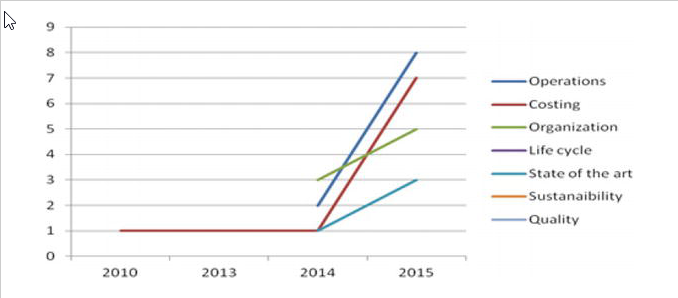
\includegraphics[scale=0.7]{images/publicacionesgestion.png}
\caption{Número de publicaciones por año y según temática \citep{fera2018}}
\end{figure}

El primer punto de partida para ser desarrollado en el futuro está enfocado, principalmente, en la definición de modelos de la contabilidad de costo, y también en el modelo de programación para manufactura asistida.
El costo total de fabricación para cada geometría es obtenido a través de la suma de costos por cada paso. 


$$C_{tot}(G_i)=C_{prep}(G_i)+C_{buidjob}(G_i)+C_{setup}(G_i)+C_{build}(G_i)+C_{removal}(G_i)$$ 

Donde:

\begin{itemize}
\item[$ $] $C_{tot} $ es el costo total de fabricación por cada parte con i-ésima geometría [\$/pieza]
\item[$ $] $G_i $ es la iésima geometría.
\item[$ $] $C_{prep} $ es el costo de preparación de los datos de la geometría (orientación, soportes, estructuras, etc.)[\$/pieza]
\item[$ $] $C_{build} $ es el costo de trabajo de ensamblaje y construcción [\$/pieza].
\item[$ $] $C_{setup} $ es el costo de seteo de la máquina [\$/pieza].
\item[$ $] $C_{build} $ es el costo de construcción de una pieza con una i-ésima geometría [\$/pieza].
\item[$ $] $C_{removal} $ Costo de remoción de la pieza con i-ésima geometría desde la cámara de la máquina [\$/pieza].
\end{itemize}

EL primer paso del proceso presentado en este documento son los datos del diseño de la geometría, que incluye orientación y estructura de soporte generada. Una posible formulación para este costo considera el valor específico del costo referido al número de partes producidas, por cada geometría.  

$$C_{prep}(G_i)=(C_{op.pre}+C_{PC})\cdot \frac{T_{prep}(G_i)}{N_i}$$

Donde:

\begin{itemize}
\item[$ $] $C_{prep} $ costo de preparación de los datos de geometría (orientación, estructuras de soporte, etc)[\$/pieza] 
\item[$ $] $G_i $ es la i-ésima geometría. [-]
\item[$ $] $C_{op.pre} $ Tarifa por hora del operador de pre-proceso  [\$/hora]
\item[$ $] $C_{PC} $ Tarifa por hora del espacio de trabajo, incluido costos requeridos de software y herramientas [\$/hora].
\item[$ $] $T_{prep} $ Tiempo requerido para preparar los datos de CAD [h].
\item[$ $] $N_i$ Cantidad de piezas con i-ésima geometría [-]
\end{itemize}

Cuando las actividades previas, es decir, la preparación de la geometría y la fase de planificación, están completas, comienza la fase de producción. Este proceso incluye la importación de los datos y la configuración de la máquina. Durante esta fase, la máquina no debe estar en uso, es por esta misma razón que se incluye el costo horario. También, en este caso, se usó el volumen de las piezas como un criterio de distribución en la formulación final. Así:


$C_{setup}(G_i)=(C_{op.mach}+C_{mach})\cdot(T_{setup}+(F_{mat.ch}\cdot T_{mat.ch})\cdot F_{inertgas}\cdot \frac{V(G_i}{\sum_{i=1}^{n} V(G_i)\cdot N_i}$

Donde:

\begin{itemize}
\item[$ $] $C_{setup} $ es el costo de configuración de la máquina [\$/pieza]
\item[$ $] $G_i $ i-ésima geometría[-]
\item[$ $] $C_{op.mach} $ tarifa por hora del operario de la máquina [\$/hora]
\item[$ $] $C_{mach} $ costo por hora de máquina [\$/hora]
\item[$ $] $T_{setup} $ Tiempo requerido por la configuración de la máquina [h]
\item[$ $] $F_{mat-ch} $ Factor para modelar la frecuencia del cambio de material [-]
\item[$ $] $T_{mat.ch} $ Tiempo requerido para el cambio de material [h]
\item[$ $] $F_{intertgas} $ Factor para modelar el esfuerzo requerido por manipular en ambiente protector de gases.
\item[$ $] $V $ es el volumen de la geometría.
\item[$ $] $N_i$ Cantidad de piezas para cada i-ésima geometría [-].


\end{itemize}

En la fórmula anterior, es posible incluir el tiempo extra de trabajo debido al uso de gas protector ($F_{inertgas}$), el cual es un factor que puede ser 1 o 0. También, el cambio de material puede ser considerado a través de un factor que, al igual que el anterior, puede ser 1 o 0 ($F_{mat.ch}$). Además, si el costo está dividido en más trabajos, esta formulación puede ser utilizada como una fracción.
El costo por hora de la máquina se obtiene dividiendo el costo de compra de ésta por el periodo de depreciación de la máquina, y su tiempo de actividad por año. 

\begin{equation*}
C_{machine}=\frac{Cost_{machine}}{h\cdot upt}
\end{equation*}

Donde:

\begin{itemize}
\item[$ $] $C_{machine}$ es el costo por hora de la máquina [\$/h]
\item[$ $] $Cost_{machine}$ es el costo de compra de la máquina [\$]
\item[$ $] $h$ es el periodo de depreciación de la máquina [Años]
\item[$ $] $upt$ es el tiempo de actividad de la máquina [horas/año]

\end{itemize}

A continuación, se muestra la fórmula para el cálculo de los pasos de construcción de las piezas. En esta fase, se considera la fabricación de todas las piezas en la cámara. EL costo considera:
\begin{itemize}
\item Máquina
\item Energía
\item Material
\item Gas
\end{itemize}


$$C_{build}=T_{build}(G_i)\cdot(C_{mach}+C_{inertgas}\cdot Gas_{cons}+C_{energy}*P_{cons}\cdot K_u)+M(G_i)\cdot (C_{material}\cdot W_f)$$


Donde:

\begin{itemize}
\item[$ $] $C_{build}$ es el costo de construcción de una pieza con i-ésima geometría [\$/pieza]
\item[$ $] $G_i$ es la i-ésima geometría [-]
\item[$ $] $T_{build}$ es el tiempo total de construcción [horas]
\item[$ $] $C_{machine}$ es el costo por hora de la máquina [\$/hora]
\item[$ $] $C_{inertgas}$ es el costo del gas inerte [\$/$m^3$]
\item[$ $] $Gas_{cons}$ es el consumo promedio de gas [$m^3$/hora]
\item[$ $] $C_{energy}$ es el costo de energía [\$/KWh]
\item[$ $] $P_{cons}$ es la potencia consumida [kW]
\item[$ $] $M$ es la masa de la geometría [kg]
\item[$ $] $C_{material}$ es el costo del material [\$/kg]
\item[$ $] $W_f$ es el factor de desecho para el polvo [-]
\end{itemize}

Cuando la operación de construcción concluye, es necesario remover las piezas fabricadas y el sustrato desde la cámara de la máquina. De la misma forma, en este caso se incluye el factor de modelo, esto es considerar el tiempo extra de esfuerzo por trabajar en un ambiente gas protector. EL criterio de localización para este costo está basado en el volumen de las piezas.

\begin{equation*}
C_{rem}(G_i)=T_{rem}\cdot (C_{op.mach}+C_{mach})\cdot\frac{V(G_i}{\sum_{i=1}^{n} V(G_i)\cdot N_i}\cdot F_{inertgas} 
\end{equation*}
Donde:

\begin{itemize}
\item[$ $] $C_{rem} $ es el costo de remoción de la pieza con i-ésima geometría desde la cámara [\$/pieza]
\item[$ $] $G_i $ i-ésima geometría[-]
\item[$ $] $T_{rem} $ Tiempo requerido para remover la pieza desde la cámara de la máquina [\$/hora]
\item[$ $] $C_{op.mach} $ Tarifa horaria del operador de la máquina [\$/hora]
\item[$ $] $C_{mach} $ Costo por hora de la máquina [\$/hora]
\item[$ $] $F_{intertgas} $ Factor para modelar el esfuerzo requerido por manipular en ambiente protector de gases.
\item[$ $] $V $ es el volumen de la geometría.
\item[$ $] $N_i$ Cantidad de piezas para cada i-ésima geometría [-].
\end{itemize}

El problema de la programación en la fabricación aditiva, diferente a la programación tradicional de máquinas, ha sido un desafío a resolver desde que esta tecnología comenzó a ser parte permanente dentro de los entornos de producción en diferentes empresas, especialmente en el campo de la defensa y la industria aeroespacial. La pregunta que se busca responder es común en todos los problemas vinculados a la programación de los procesos, es decir: \textit{¿cuál es la programación que permite respetar las fechas de producción con el menor costo?}.
Si bien la pregunta es la misma, el contexto de la fabricación aditiva es muy diferente al de producción tradicional, ya que la actividad se realiza durante toda la fase de diseño y transferencia de datos desde la estación de trabajo; además, se nota el hecho que con la manufactura aditiva es posible producir varios y complejos tipos de geometrías en la misma ejecución de la producción. Por esta razón, se debe introducir un modelo "multiobjetivo" para la programación.
El marco de trabajo del desarrollo es parecido a los problemas tradicionales de la programación de la producción pero, en este caso, las órdenes de producción son entradas para la máquina de fabricación aditiva.
\begin{figure}[H]
\centering
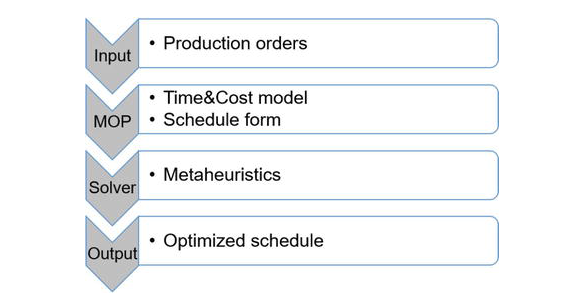
\includegraphics[scale=0.8]{images/mapaproduccion.png} 
\caption{Marco de trabajo para la programación de la producción \citep{fera2018}}
\end{figure}

 Además, cada orden es caracterizada según los siguientes atributos:\\

\begin{table}[H]
\centering

\begin{tabular}{|c|c|c|}

\hline
Atributo & Descripción & unidades\\
\hline 
$d_1$ & demanda de la i-ésima geometría  & [pieza] \\ 
\hline 
$dd_1$ & fecha límite para la i-ésima geometría & [día] \\ 
\hline 
$V_1$ & Volumen de la i-ésima geometría & [$cm^3$] \\ 
\hline 

\end{tabular} 
\caption{Atributos y descripción para programación de la producción en máquinas de fabricación aditiva \citep{fera2018}.}
\end{table}

Una vez que se listan los atributos para las órdenes de producción, se debe señalar que para  este caso se aplicará un modelo de tiempo y costo. Particularmente, se debe considerar el tiempo total o tiempo para producir una unidad de la i-ésima geometría (CT) y el costo total de la pieza (TPC).



\end{description}






\begin{description}
\item \textbf{Conclusiones:} Se pudo realizar el intento de analizar y categorizar los temas relacionados con los problemas de producción de la fabricación aditiva. Esta tecnología comenzó a transformarse en una solución industrial reciente y, entonces, esta fue reconocida como una interesante temática con la posibilidad de profundizar la investigación en el área, acaso estas tecnologías logran un buen nivel de madurez en términos de la resistencia mecánica, y sus tolerancias. Después de este primer paso de análisis, el estado de las investigaciones acerca de la gestión de las operaciones en el campo fue analizada y estudiada. Este capítulo define un camino preciso para la revisión de la literatura, y es analizada y categorizada con el método mencionado anteriormente.
Del análisis de la literatura realizado, fue bastante claro desde la tecnología y de los niveles de calidad en la producción, y no son muchos los problemas abiertos, por tanto es posible concluir que la fabricación aditiva está lo suficientemente lista como para ser llevada al contexto industrial, dándole algunos ajustes que aún siguen necesitando para evitar problemas en la porosidad, tolerancias en la concentricidad y circularidad de las piezas trabajadas. Sin embargo, las piezas en mntal pueden ser fabricadas directamente utilizando la manufactura aditiva, teniendo un buen nivel de confiabilidad de éstas,cuando es sometida a esfuerzos de tensión. La fabricación aditiva está evolucionando, así también la necesidad de entender los problemas en la gestión de la producción. No obstante, es posible decir esto teniendo en cuenta que desde el punto de vista de las propiedades mecánicas y sus propiedades existe una variedad de trabajos; pero no se puede decir lo mismo desde el punto de vista de la gestión. Así, este estado del arte puede identificarse como el primer punto de estudio en una importante problemática acerca de los métodos de medición y los procesos de coste cuando la manufactura aditiva es utilizada. Sumado a esto, la temática de la gestión se ve afectada desde una ausencia importante respecto a la información disponible.  No obstante, una gran variedad autores han comenzado a estudiar la problemática de la gestión relacionada a sistemas generales, pero ninguno reconoce un límite principal en el nivel de conocimiento actual. Finalmente, en este documento fue presentado un modelo de asignación de costos que encaja con los requerimientos de esta nueva tecnología, así también formulaciones matemáticas para la programación de una máquina única de fabricación aditiva.   

\end{description}

\section{Gestión del mantenimiento basado en la teoría de la confiabilidad}



Cruz, B. (2018). Aplicación de modelo RCM bajo las normas SAE JA1011 y JA1012 para mejorar la gestión del mantenimiento en la máquina flexoplegadora de cartón Martin 618. Universidad de Santiago de Chile.

\begin{description}
\item \textbf{Objetivos:} Diseñar una propuesta basada en RCM para la máquina flexoplegadora de cartón MARTIN 618 que mejore los indicadores de confiabilidad y mantenibilidad, conforme a un plan para la gestión del activo desde el foco de mantenimiento. 

\end{description}

\begin{description}
\item \textbf{Resumen:} El uso de la metodología del mantenimiento centrado en la confiabilidad (RCM) contempla no solamente el estudio del equipo como tal sino de los subsistemas que lo conforman y la interacción con el entorno físico que lo rodea. 
En esta tesis primero se realizó la identificación de los subsistemas que tienen mayor incidencia en las fallas y en la prolongación de estas, aplicando un análisis de Pareto se reconocen aquellos subsistemas críticos para la producción, para luego estudiar caso a caso las fallas potenciales a través de un análisis de modos y efectos de falla (AMEF). Al definir los modos y las causas de las fallas se pudo establecer un catálogo de fallas completo para cada subsistema, en donde se condensa información relevante en cuanto a criticidad de cada una ellas y el impacto en las metas de producción, mantenimiento, salud y medio ambiente; así como su priorización. Luego, mediante el desarrollo de la hoja de decisión RCM, con ayuda del árbol lógico, se determinaron las siguientes estrategias de mantenimiento para eliminar las causas de las fallas identificadas: 
\begin{itemize}
\item Optimización del mantenimiento preventivo.
\item Implementación de mantenimiento predictivo.
\item Optimización del cambio sistemático de componentes en función de la frecuencia de las fallas.
\item Implementación de inspecciones sensoriales por parte de los operadores.
\item Identificación de mejoras en las instalaciones a cargo de Ingeniería de Mantenimiento.
\item Identificación de repuestos críticos.

\end{itemize}
   
Como resultado de la aplicación de la metodología se espera lograr incrementar la vida útil de los componentes de los equipos, así como la disponibilidad de los mismos al disminuir las fallas y sus consecuencias, incrementando así la confiabilidad operacional del activo significando mayores beneficios económicos para la empresa. 
 
       
\end{description}

\begin{description}
\item \textbf{Resultados:} El activo seleccionado para este estudio muestra indicadores de seguridad operacional bastante desfavorables, una disponibilidad porcentual de un 42.8\% desde ningún punto de vista es concebible económicamente para una empresa, menos para una que, como es el caso de packaging CMPC chile, pretende ser líder en excelencia operacional a nivel internacional. Para complementar esto, el diagrama de Jack Nife es revelador para indicar la posición que tiene el equipo en comparación con sus similares dentro del proceso productivo. Sugiriendo indudablemente que es necesario confrontar el problema y dar un paso hacia adelante en la gestión del activo. Es por eso que un estudio RCM es la mejor manera de dilucidar los principales problemas que están aquejando el funcionamiento de la máquina flexoplegadora MARTIN 618.
 Con la interpretación del diagrama de Pareto, establecimos que los focos estarían centrados en la plegadora, rapidset y slotter, con este primer paso sacamos provecho de abordar el 70 \% de los objetivos, que para nuestro caso resultaría en un aumento de la confiabilidad y disponibilidad del equipo si logramos administrar las tareas de mitigación. Estos objetivos son las fallas que provocan intervenciones de emergencia deteniendo el activo mientras está produciendo. El segundo análisis de Pareto nos profundiza el estudio dando oportunidad de desentrañar los problemas desde su causa raíz, siendo este uno de los objetivos principales de la metodología evitando caer en redundancias o ineficiencia de las tareas por realizar un estudio demasiado superficial. 
 
 \begin{figure}[H]
 \centering
 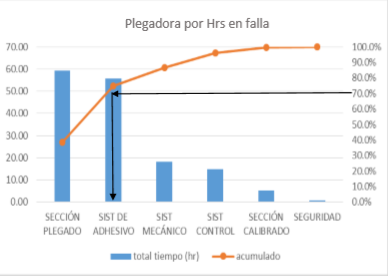
\includegraphics[scale=0.8]{images/plegadorapareto.png}
 \caption{Diagrama de Pareto por número de fallas para Plegadora \citep{cruz2018}}
 \end{figure}
 
Las fallas en los sistemas generalmente son aleatorias y su probabilidad de ocurrencia pueden ser modeladas a través de diversos métodos matemáticos. Para la confiabilidad operacional la que más se adapta es la distribución de Weibull y al obtener el comportamiento de cada subsistema podemos establecer metas de confiabilidad o límites a los cuales la empresa está dispuesta a trabajar. Si observamos las curvas de confiabilidad de cada uno de los subsistemas críticos, tenemos que para la sección de plegado, el sistema de adhesivo y el árbol de ranurado a las 200 horas de funcionamiento tendrían una probabilidad de funcionamiento del 55 \% lo que es muy bajo para una empresa de excelencia operacional, para el grupo de tinta y la lona de aspiración a las mismas 200 horas de funcionamiento presentan una probabilidad cercana al 64 \% de confiabilidad.  

\begin{figure}[H]
\centering
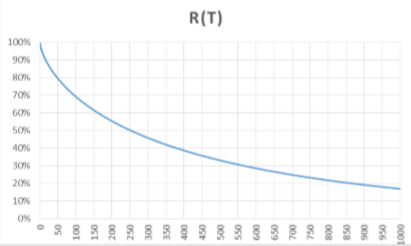
\includegraphics[scale=0.8]{images/plegadoraconf.png}
\caption{Curva de confiabilidad para la sección de plegado \citep{cruz2018}}
\end{figure}

\begin{figure}[H]
\centering
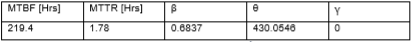
\includegraphics[scale=0.9]{images/plegadoraind.png}
\caption{Indicadores de mantenimiento para la sección de plegado \citep{cruz2018}}
\end{figure}

\end{description}

\begin{description}
\item \textbf{Conclusiones:} El presente estudio RCM pretende brindar herramientas y conocimientos para la gestión de la instalación y con esto implementar un programa eficaz de mantenimiento, logrando llevar a la empresa a la excelencia operacional que está buscando, aumentando la confiabilidad y mantenibilidad de sus equipos y otorgando grandes beneficios económicos. 
Claramente la metodología no debe terminar acá, sino que debe seguir un proceso constante. Ciertamente los principales problemas de hoy no serán los mismos de mañana si es que se logra satisfacer las necesidades que justificaron en primer lugar este análisis. Es indudable que el proceso debe seguir a través del tiempo y que debe involucrar a cada integrante del ciclo de producción. 
\end{description}




\section{Tecnologías innovadoras que utilicen CMMS para la gestión del mantenimiento.}

Aransyash, D., Rosa, F., and Colombo, G. (2019). Smart maintenance: A wearable augmented reality application integrated with cmms to minmize unsheduled downtime. Computer-Aidded Design and Applications.


\begin{description}
\item \textbf{Objetivos:}
\begin{itemize}
\item Mostrar la integración de un sistema de información de activos como un CMMS con el sistema de realidad aumentada.
\item Demostrar cómo la información integrada de activos de un CMMS con la tecnología de realidad aumentada puede reducir la indisponibilidad.
\end{itemize}
\end{description}

\begin{description}
\item \textbf{Resumen:} El objetivo final de los encargados del mantenimiento en cualquier industria es maximizar el tiempo de actividad de la producción y mantener la indisponibilidad de los activos al mínimo. Estos factores afectan la capacidad de la industria para cumplir los plazos de producción, sin dejar de garantizar la buena calidad de los productos manteniendo los costos de producción al mínimo. Para lograr este objetivo, se requieren herramientas innovadoras y métodos efectivos del mantenimiento. Estudios previos muestran que el crecimiento de la complejidad de las tecnologías de manufactura actual necesitarán incrementar las competencias, así como la capacitación del personal para resolver rápidamente las interrupciones que ocurren. Así, es difícil lograr una operación de reparación eficiente, especialmente cuando un fallo funcional de la máquina involucra varios posibles problemas, así como la asignación  de las habilidades técnicas y fuentes para atender el fallo de equipo requieren más que solo la información reportada por el operador. La realidad aumentada es una de las tecnologías que emergen en el marco de trabajo de la Industria 4.0, que provee un camino para acelerar el proceso de mantenimiento y minimiza el servicio del trabajo de mantenimiento debido a la información limitada entregada por el operador.     
\end{description}

\begin{description}
\item \textbf{Resultados:} El desarrollo de un sistema RA-CMMS para el mantenimiento fue demostrado en una impresora 3D, la cual es una tecnología emergente que transformará el cómo los productos serán fabricados en el futuro. Debido al avance que subyace en esta tecnología, el mal funcionamiento de una impresora 3D puede ser causada por diversas fuentes. En este estudio, se consideran dos tipos de fallas: fallas que involucren un componente que se puede reparar, y fallas que requieren cierta experiencia para resolver el problema. Los pasos para desarrollar el sistema RA-CMMS son los siguientes: la relación entre los diferentes componentes fue diseñada para un almacenamiento eficiente de de un alto volumen de datos.

\begin{figure}[H]
\centering
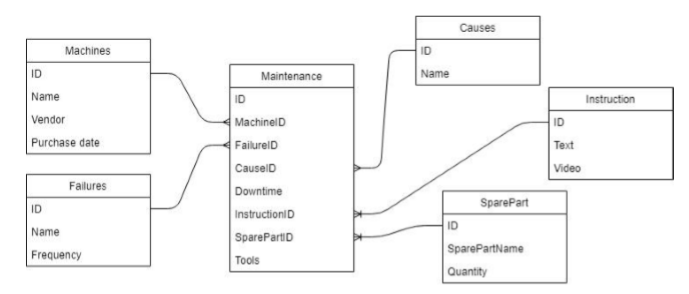
\includegraphics[scale=0.7]{images/umla.png}
\caption{Diagrama UML que describe la relación de los registros entre máquinas, fallas, causas y acciones de mantenimiento \citep{aransyash2019}}
\end{figure}




En segundo lugar, la interfaz de usuario fue diseñada para presentar la información relevante del activo. Por ejemplo, las instrucciones de mantenimiento pueden ser presentadas en formato de texto o mensajes verbales, seguidos por etiquetas para determinar con precisión la localización del objetivo con animaciones 3D o vídeos. La interacción con la interfaz del usuario fue realizada según la visión del usuario hacia el objeto, y el reconocimiento de comandos se realiza con gestos manuales o a través de la voz, con el objetivo de navegar en el menú o el control de contenidos digitales. El objetivo a través de la realidad aumentada (es decir, la imagen objetivo), es anexada a la impresora 3D para entrega la localización en la cual el contenido digital debe ser puesto según el marco de referencia en la visión del usuario. Así, el usuario puede acceder a la funcionalidad a través de la aplicación de Realidad aumentada para el diagnóstico de las tareas, o crear ordenes de trabajo utilizando un teclado inalámbrico. Cuando ocurre una falla inesperada, el operador puede hacer un reporta a través del comando de voz o puede observar el tipo de falla y las posibles causas.

\begin{figure}[H]
\centering
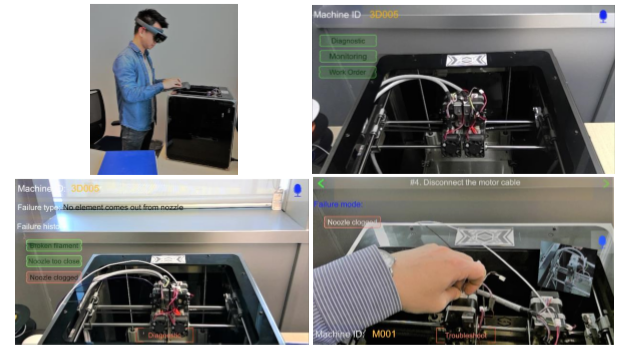
\includegraphics[scale=0.7]{images/arsistema.png}
\caption{Sistema de Realidad Aumentada integrado con CMMS. De izquierda a derecha y de arriba a abajo: (a) operador utiliza el sistema utilizando teclado inalámbrico; (b) funcionalidad del sistema; (c) operación de diagnóstico basado en el historial de fallas; (d) guía del sistema al operador a través de instrucciones de texto y video \citep{aransyash2019}.}
\end{figure} 
\end{description}

\begin{description}
\item \textbf{Conclusiones:} El propósito principal de los sistemas de Realidad aumentada y la integración a través de CMMS es establecer una aproximación más efectiva para tratar con las paradas inesperadas en el contexto cotidiano de la industria, la cual es caracterizada por la complejidad, conectividad y diversidad del sistema de producción. A través de la obtención de información completa sujeta a la información de los activos y las buenas prácticas de las acciones de mantenimiento en el ambiente de la realidad aumentada, esta aproximación puede asistir al operador no capacitado, para diagnosticar instantáneamente, o reparar cualquier falla del equipo, minimizando el tiempo de reparación no programado. Además, la inspección inmediata de los activos con fallas en sus funciones puede ayudar a idear una planificación de mantenimiento más precisa y, de este modo, evitar las operaciones de mantenimiento no productivos. La reducción del tiempo de recuperación podrá mejorar la disponibilidad de los equipos y, por lo tanto, incrementar la rentabilidad y la ventaja competitiva en la industria.
\end{description}
